\chapter{Mengenal Python dan Anaconda}

\section{Teori}
\subsection{Jenis-Jenis Variabel}
Variabel merupakan tempat penyimpanan data. Tipe data merupakan jenis data yang tersimpan di dalam variabel. terdapat aturan dalam penulisan Variabel.
\begin{enumerate}
 \item Nama variabel diawali dengan huruf atau garis bawah, contoh: nama, \_nama, namaKu, nama\_variabel.
 \item Karakter selanjutnya dapat berupa huruf, garis bawah atau angka, contoh: \_\_nama, nama1, p1.
 \item Karakter bersifat case-sensitive (huruf besar dan huruf kecil dibedakan), contoh: Nama dan NAMA keduanya adalah variabel yang berbeda.
 \item Nama variabel tidak boleh menggunakan kata kunci yang ada pada bahasa pemrograman python, contoh: if, else, while
 \item Nama variabel tidak boleh diawali dengan angka
\end{enumerate}

Jenis-jenis tipe data pada python.
Tipe Data Primitif, dibagi menjadi 3 yaitu:
\begin{enumerate}
 \item Tipe data integer (angka), penulisannya tidak membutuhkan tanda petik, contoh: 10 atau 15
 \item Tipe data string (teks), tipe data string ditandai dengan teks yang diapit oleh tanda petik (""), contoh: "nama saya adalah dinda majesty"
 \item Tipe data boolean (memiliki dua nilai yaitu true dan false atau 0 dan 1)
\end{enumerate}

Contoh penulisan variabel dan tipe datanya:
\begin{enumerate}
 \item angka = 10, angka merupakan nama variabel sedangkan 10 adalah nilai dari variabel yang tipe datanya integer.
 \item nama = "Dinda Majesty", nama merupakan nama variabel sedangkan "Dinda Majesty" merupakan nilai dari variabel yang tipe datanya string, ditandai dengan adanya petik ("").
 \item makan = True , makan merupakan nama variabel sedangkan True merupakan nilai dari variabel yang tipe datanya boolean.
\end{enumerate}

\subsection{Input dan Output}
Berikut kode untuk meminta inputan dari user.
\lstinputlisting[caption=Input dan Output , language=Python, firstline=7, lastline=10]{src/teori.py}
Perintah input() berguna untuk meminta inputan dari user, sehingga memungkinkan user untuk menginputkan data.\\
Perintah print() berguna untuk menampilkan output dari data yang diinputkan oleh user, sehingga data yang diinputkan user dapat ditampilkan ke layar.

\subsection{Operator Aritmatika dan Konversi Tipe Data}
Operator aritmatika
\begin{enumerate}
 \item penjumlahan (+)
 \item pengurangan (-)
 \item perkalian (*)
 \item pembagian (/)
 \item sisa bagi/modulus (%)
 \item pemangkatan (**)
\end{enumerate}
Cara melakukan perubahan terhadap tipe data string menjadi integer, contoh: variabel = "10". Kita dapat mengubah string "10" menjadi angka 10 dengan menambahkan kode int(variabel), dengan begitu 10 yang awalnya bertipe data string akan dikonversikan menjadi integer.\\
Cara melakukan perubahan terhadap tipe data integer menjadi string, contoh: variabel = 150. Kita dapat mengubah integer 150 menjadi string "150" dengan menambahkan kode str(variabel), maka tipe data dari variabel akan dikonversikan menjadi string.

\subsection{Perulangan}
perulangan terdiri atas 3 kondisi.
\begin{enumerate}
 \item While, apabila kondisinya True, maka perulangan akan terus berjalan hingga diperoleh kondisi False. Contoh penggunaan while:\\
\lstinputlisting[caption=While Loop , language=Python, firstline=12, lastline=18]{src/teori.py}
 \item For, perulangan for bisa melakukan perulangan terhadap item apapun seperti list atau string. Contoh penggunaan For:\\
\lstinputlisting[caption=For Loop , language=Python, firstline=20, lastline=23]{src/teori.py}
 \item nested, perulangan ini memungkinkan adanya perulangan didalam perulangan. Contoh penggunaan nested:\\
\lstinputlisting[caption=Nested Loop , language=Python, firstline=25, lastline=35]{src/teori.py}
\end{enumerate}
Pada penulisan sintaks While dan For harus memperhatikan identasi (baris yang menjorok ke dalam), jika tidak diperhatikan dengan baik maka akan terjadi error terhadap identasi. Untuk menambahkan identasi dapat menggunakan spasi atau tab.

\subsection{IF Statement}
kondisi if dapat digunakan didalam looping dan dapat digunakan untuk memberikan kondisi tertentu dengan cara mengetikkan if lalu kondisi yang akan terjadi.\\
\begin{enumerate}
 \item if hanya menjalankan satu kondisi dan menampilkan satu output. Contoh: kondisi dimana variabel a lebih besar dari variabel b, maka tampilkan hasil bahwa a lebih besar dari b.
\lstinputlisting[caption=if Statement , language=Python, firstline=37, lastline=41]{src/teori.py}
 \item elif digunakan apabila kondisi pertama tidak benar maka lakukan kondisi lain (alternatif). Contoh: kondisi dimana variabel a sama dengan variabel b, maka jika b lebih besar dari a, tampiilkan hasil b lebih besar dari a, namun jika a dan b bernilai sama, maka tampilkan a sama dengan b
\lstinputlisting[caption=Elif , language=Python, firstline=43, lastline=49]{src/teori.py}
\item else digunakan apabila kondisi yang terjadi bernilai salah, maka lakukan else. Contoh: kondisi dimana variabel a lebih besar dari variabel b, maka jika b lebih besar dari a, tampiilkan hasil b lebih besar dari a, jika a dan b bernilai sama, maka tampilkan a sama dengan b, jika salah maka tampilkan a lebih besar dari pada b
\lstinputlisting[caption=Else , language=Python, firstline=51, lastline=59]{src/teori.py}
\item Nested if merupakan if didalam if (if bersarang), terdapat dua if didalam satu kondisi. Contoh: variabel x sama dengan 41, kondisi pertama yaitu jika x besar dari 10 maka tampilkan lebih besar dari 10, kondisi kedua yaitu jika x besar dari 20, maka tampilkan lebih besar dari 20, jika salah maka tampilkan tidak melebihi 20.
\lstinputlisting[caption=Nested If , language=Python, firstline=61, lastline=69]{src/teori.py}
\end{enumerate}

\subsection{Error}
\begin{enumerate}
 \item NameError, terjadi apabila kode mengeksekusi nama yang tidak terdefenisikan. Contoh:
 \begin{verbatim}
 nama = "Dinda Majesty"
 print(Nama)
 \end{verbatim}
 Maka akan menghasilkan output NameError: name 'Nama' is not defined. error ini dapat diatasi dengan mengubah variabel yang di print sesuai dengan variabel yang didefenisikan, karena penulisan pada pyton bersifat case-sensitive
 
 \item SyntaxError, terjadi apabila kode python mengalami kesalahan saat penulisan. Contoh: menuliskan variabel yang didahului angka (1nama = "Dinda Majesty") maka akan muncul eror SyntaxError: invalid syntax. error ini dapat diatasi dengan memperhatikan tata cara penulisan kode pada bahasa pemrograman python.
 
 \item TypeError, terjadi apabila kode melakukan operasi atau fungsi terhadap tipe data yang tidak sesuai. Contoh: melakukan penjumlahan terhadap tipe data string dan integer. eror ini dapat diatasi dengan mengubah tipe data string menjadi integer.
 \begin{verbatim}
 a = "10"
 b = 5

 print(a + b)
 \end{verbatim}
 Maka akan menghasilkan output eror TypeError: can only concatenate str (not "int") to str
 
 \item IdentationError, terjadi apabila kode perulangan atau pengkondisian tidak menjorok kedalam (tidak menggunakan identasi), error ini dapat diatasi dengan menambahkan tab atau spasi. Contoh:
 \begin{verbatim}
 a = 200
 b = 330
 if b > a:
 print("b lebih besar dari a")
 \end{verbatim}
 Maka akan menghasilkan output eror IndentationError: expected an indented block
\end{enumerate}

\subsection{Try Except}
Try Except merupakan perintah yang bisa digunakan dalam penanganan error pada bahasa pemrograman python. perintah ini biasanya digunakan saat penanganan error input/output, operasi database, pengaksesan indeks suatu list atau dictionary dan berbagai kasus lainnya.\\
Contoh sederhana penggunaan Try-Except saat menangani NameError
\lstinputlisting[caption=Try Except , language=Python, firstline=71, lastline=77]{src/teori.py}
Pada contoh diatas, try except akan menghasilkan output Variabel x tidak ada, karena kita tidak mendefinisikan variabel x sebelum kita menampilkan output x ke layar. Dengan menggunakan try except kode yang kita buat terhindar dari error dan kita bisa mengetahui kesalahan yang terjadi ketika terdapat error pada kode kita.

\section{Keterampilan Pemrograman}
\subsection{Modulus}
\lstinputlisting[caption=Modulus, language=Python, firstline=7, lastline=24]{src/1184011.py}
\subsection{Hello NPM}
\lstinputlisting[caption=Hello NPM, language=Python, firstline=26, lastline=32]{src/1184011.py}
\subsection{Hello NPM (3 Digit Belakang)}
\lstinputlisting[caption=3 Digit Belakang, language=Python, firstline=34, lastline=42]{src/1184011.py}
\subsection{Hello NPM (Digit ke-3)}
\lstinputlisting[caption=Digit ke-3, language=Python, firstline=44, lastline=48]{src/1184011.py}
\subsection{Variabel Alfabet}
\lstinputlisting[caption=Variabel Alfabet, language=Python, firstline=50, lastline=58]{src/1184011.py}
\subsection{Penjumlahan NPM}
\lstinputlisting[caption=Penjumlahan NPM, language=Python, firstline=60, lastline=71]{src/1184011.py}
\subsection{Perkalian NPM}
\lstinputlisting[caption=Perkalian NPM, language=Python, firstline=73, lastline=84]{src/1184011.py}
\subsection{Print Vertical}
\lstinputlisting[caption=Print Vertical, language=Python, firstline=86, lastline=90]{src/1184011.py}
\subsection{Digit Genap NPM}
\lstinputlisting[caption=Digit Genap NPM, language=Python, firstline=92, lastline=99]{src/1184011.py}
\subsection{Digit Ganjil NPM}
\lstinputlisting[caption=Digit Ganjil NPM, language=Python, firstline=101, lastline=108]{src/1184011.py}
\subsection{Bilangan Prima NPM}
\lstinputlisting[caption=Bilangan Prima NPM , language=Python, firstline=110, lastline=126]{src/1184011.py}

\section{Keterampilan Penanganan Error}
\subsection{Peringatan Error dan Cara Mengatasinya}
\begin{enumerate}
 \item IndentationError: expected an indented block, terjadi apabila kode perulangan atau pengkondisian tidak menjorok kedalam (tidak menggunakan identasi), error ini dapat diatasi dengan menambahkan tab atau spasi.
 \item TypeError: can only concatenate str (not "int") to str, terjadi apabila kode melakukan operasi atau fungsi terhadap tipe data yang tidak sesuai. Contoh: melakukan penjumlahan terhadap tipe data string dan integer. eror ini dapat diatasi dengan mengubah tipe data string menjadi integer.
 \item NameError: name 'NOM' is not defined, error ini dapat terjadi apabila terdapat kesalahan penulisan dan saat dijalankan, tidak ditemukan name NOM didalam kode yang dituliskan. error ini dapat diatasi dengan memperhatikan penulisan kode. 
 \item SyntaxError: invalid syntax, error ini terjadi apabila kode yang dijalankan memiliki kesalahan penulisan syntax. Contoh: if(prima=True): salah karena kekurangan tanda =, seharusnya ditulis if(prima==True):, error ini dapat ditangani dengan memperhatikan penulisan kode program
\end{enumerate}
\subsection{Percobaan Try Except}
\lstinputlisting[caption=Bilangan Prima NPM , language=Python, firstline=7, lastline=15]{src/2rr.py}
Output:
\begin{figure}[H]
    \centering
    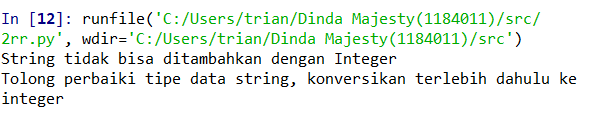
\includegraphics[scale=1]{figures/tryexcept}
    \caption{\textit{Try Except}}
    \label{Try Except}
\end{figure}